\section{Equazione del calore e la sua approssimazione numerica}
L'equazione del calore, come facilmente intuibile, è stata formulata per determinare l'evoluzione di un sistema isolato che presenta al suo interno una data distribuzione di calore.\\
Euristicamente, non è difficile pensare che si possano codificare (pensando ad un'immagine in bianco e nero) i pixel più luminosi come punti \textit{"più caldi"}, mentre quelli più scuri come punti \textit{"più freddi"} ed applicare così l'equazione del calore all'immagine.\\
Mediante uno script MATLAB si può dunque osservare come quest'ultima operi nella pratica, sfruttando una approssimazione alle \textbf{differenze finite } utile per il calcolo delle derivate.\\
\subsection{Metodo delle differenze finite}
Il metodo delle differenze finite, come anticipato, viene impiegato nel calcolo approssimato delle derivate. Data una generica funzione u, consideriamone lo sviluppo di Taylor\\
\vspace{0.25em}
\centering
$u(x_i+\Delta(x))=u(x_i)+u'(x_i)\Delta(x)+\frac{1}{2}u''(x_i)\Delta(x)^2+o(h^2)$ \\
\vspace{0.25em}
\raggedright
La scelta adottata per la suddetta approssimazione risulterà dunque essere:\\
\vspace{0.25em}
\centering 
$\frac{du}{dx}\approx\frac{u(x+\Delta(x))-u(x)}{\Delta(x)} \approx \frac{u_{i+1} - u_i}{\Delta(x)} $.
\cite{FD}\\
\vspace{0.25em}
\raggedright
Tale approssimazione è detta \textbf{differenza finita in avanti}. Analogamente si trova, come approssimazione altrettanto valida la \textbf{differenza finita all'indietro}:\\
\vspace{0.25em}
\centering 
$\frac{du}{dx}\approx\frac{u(x)-u(x-\Delta(x))}{\Delta(x)} \approx \frac{u_i - u_{i-1}}{\Delta(x)} $.\\
\vspace{0.25em}
\raggedright
Consideriamo adesso gli sviluppi di Taylor che hanno portato a queste due approssimazioni e sottraiamo membro a membro.\\
\vspace{0.25em}
\centering
$u(x_i+\Delta(x))=u(x_i)+u'(x_i)\Delta(x)+\frac{1}{2}u''(x_i)\Delta(x)^2+\frac{1}{6}u'''(x_i)\Delta(x)^3+o(h^3)$ \\
\vspace{0.25em}
$u(x_i-\Delta(x))=u(x_i)-u'(x_i)\Delta(x)+\frac{1}{2}u''(x_i)\Delta(x)^2-\frac{1}{6}u'''(x_i)\Delta(x)^3+o(h^3)$ \\
$\Downarrow$\\
$u(x_i+\Delta(x))-u(x_i-\Delta(x))=+2u'(x_i)\Delta(x)+2\frac{1}{6}u'''(x_i)\Delta(x)^3+o(h^3)$ \\
\vspace{0.25em}
\raggedright
\newpage
Questi conti inducono l'approssimazione:\\
\vspace{0.25em}
\centering 
$\frac{du}{dx}\approx\frac{u(x+\Delta(x))-u(x-\Delta(x))}{2\Delta(x)} \approx \frac{u_{i+1} - u_{i-1}}{2\Delta(x)}$.\\
\vspace{0.25em}
\raggedright
Tale approssimazione è detta \textbf{differenza finita centrata}.


\vspace{1em}
\raggedright
Dal momento che la derivata seconda coincide con la derivata della derivata prima, allora quest'ultima può essere approssimata nel seguente modo:\\
\centering    
{\large
\begin{align*}
\frac{d^2u}{dx^2} \approx &
\frac{
(\frac{u_{i+1} - u_i}{\Delta(x)})_{i+1} 
- 
(\frac{u_{i+1} - u_i}{\Delta(x)})_i
}{\Delta(x)}
\\
\vline
\\
= &
\frac{
\frac{(u_{i+1} - u_i)_{i+1}}{\Delta(x)} 
-   
\frac{(u_{i+1} - u_i)_i}{\Delta(x)}
}{\Delta(x)}
\\
\vline 
\\
= &
\frac{
\frac{(u_{i+2} - u_{i+1})}{\Delta(x)} 
- 
\frac{(u_{i+1} - u_i)}{\Delta(x)}
}{\Delta(x)}
\\
\vline 
\\
= &
\frac{
\frac{(u_{i+2} - u_{i+1}) 
- 
(u_{i+1} - u_i)}{\Delta(x)}
}{\Delta(x)}
\\
\vline
\\
= &
\frac{
(u_{i+2} - u_{i+1}) 
- 
(u_{i+1} - u_i)}
{\Delta(x)^2}
\\
\vline 
\\
= &
\frac{
 u_{i+2} - u_{i+1} 
-u_{i+1} + {u_i}}
{\Delta(x)^2}
.\\
\end{align*}
}
\raggedright
Per ottenere una stima accurata, è bene utilizzare un valore di $\Delta(x)$ quanto più basso possibile. La migliore è guardare la differenza tra un pixel e quello adiacente ossia $\Delta(x)=1$, ma allora 

$$\frac{d^2u}{dx^2} \approx
\frac{
 u_{i+2} - u_{i+1} 
-u_{i+1} + u_i}
{\Delta(x)^2} = u_{i+2} -2 u_{i+1} + u_i.$$

\`E chiaro che scorrendo tutti gli indici questo è equivalente a $u_{i+1} -2 u_i + u_{i-1}.$

In sintesi si può utilizzare per il calcolo del laplaciamo l'approssimazione \\
\vspace{2pt}
\centering 
$\frac{d^2u}{dx^2} \approx u_{i+1} -2 u_i + u_{i-1}$.\\
\raggedright
\newpage
\subsubsection{Errore di troncamento}

Vale la pena di fare qualche considerazione sull'errore di troncamento che si commette adottando queste approssimazioni.\\

Per definizione, l'errore è la differenza tra il valore esatto e quello approssimato. Per quanto riguarda le derivate prime basta guardare agli sviluppi di Taylor che ci hanno portato alle loro approssimazioni per osservare che\\
\begin{itemize}
    \item Differenza finita in avanti\\
    \centering
    $u(x_i+\Delta(x))=u(x_i)+u'(x_i)\Delta(x)+\frac{1}{2}u''(x_i)\Delta(x)^2+o(h^2)$ \\ $\Downarrow$\\
    $\frac{u(x_i+\Delta(x))-u(x_i)}{\Delta(x)} -u'(x_i)\approx \frac{1}{2}u''(x_i)\Delta(x)^2$\\
    \raggedright
    \item Differenza finita all'indietro\\
    \centering
    $u(x_i-\Delta(x))=u(x_i)-u'(x_i)\Delta(x)+\frac{1}{2}u''(x_i)\Delta(x)^2+o(h^2)$ \\ $\Downarrow$\\
    $\frac{u(x_i)-u(x_i-\Delta(x))}{\Delta(x)} -u'(x_i)\approx \frac{1}{2}u''(x_i)\Delta(x)^2$\\
    \raggedright
    \item Differenza finita centrata\\
    \centering
    $u(x_i+\Delta(x))-u(x_i-\Delta(x))=+2u'(x_i)\Delta(x)+2\frac{1}{6}u'''(x_i)\Delta(x)^3+o(h^3)$ \\ $\Downarrow$\\
    $\frac{u(x_i+\Delta(x))-u(x_i-\Delta(x))}{2\Delta(x)} -u'(x_i)\approx +\frac{1}{6}u'''(x_i)\Delta(x)^2$\\
    \raggedright
\end{itemize}
\vspace{2em}
Allo stesso modo, applicando la definizione di errore per la derivata seconda:

$$
\frac{d^2u}{dx^2}\vline_{x_i}-\frac{u_{i+1}-u_i}{\Delta(x)}\approx \frac{\Delta(x)^2}{2} \frac{d^2u}{dx^2}\vline_\xi.
$$

Risulta quindi evidente che l'errore dipende da $\Delta(x)^2$. 
Ad un'attenta analisi possiamo vedere che tra i metodi di approssimazione in avanti, in indietro o centrale, il calcolo dell'errore portato dai primi due sono uguali tra di loro, quello centrale invece è diverso, esso dipende da un $\Delta(x)^3$ e non da un $\Delta(x)^2$, questo vuol dire che per $\Delta(x)<1$ funziona meglio, per $\Delta(x)>1$ funziona peggio. Nel caso in analisi $\Delta(x)=1$ quindi la scelta è indifferente.
%Ma procediamo con ordine.\\

Per brevità di notazione poniamo $\Delta(x)=h$.\\
Dagli sviluppi di Taylor in $x_j$ di
$u(x_{j \pm 1}) = u(x_j \pm h)$ fino al terzo ordine, si ottiene che

$$
u''(x_j) =\frac{u(x_{j+1}) - 2u(x_j) + u(x_{j-1})}{h^2} -\frac{1}{12} u^{(4)}(\xi_j)h^2
$$

dove $\xi_j$ e un punto opportuno in $(x_{j-1} , x{j+1})$. Quindi, considerando il problema modello con condizoni di Dirichlet, per $j = 1,...,N-1$, si può scrivere che

$$
\frac{-u(x_{j+1}) + 2u(x_j) -u(x{j-1})}{h^2}
 + \frac{1}{12} u^{(4)}(\xi_j)h^2 + \sigma(x_j)u(x_j) = f(x_j) .
$$

\newpage
Introducendo la notazione $\tau_{j}=\frac{1}{12} u(4)(\xi_j)h^2$ (errore di troncamento locale) e ponendo:\\

$\boldsymbol{u}=[u_x...u_{N-1}]^T$\\
$\boldsymbol{\tau_h}=[\tau_x...\tau_{N-1}]^T$\\
$\boldsymbol{b_h}=[(f(x_1) + \frac{g_0}{h^2},f(x_2),...,f(x_{N-2}),f(x_{N-1}) + \frac{g_1}{h^2}]^T$\\

si può allora scrivere in forma matriciale,
$A_h\boldsymbol{u} = \boldsymbol{b_h} + \boldsymbol{\tau_h}$
dove $A_h = \frac{1}{h^2}
 tridiag(-1,2,-1) + diag(\sigma_1, ... ,\sigma_{N-1}) e \sigma_j = \sigma(x_j)$.\\
\vspace{1em}
Il metodo alle differenze finite consiste allora nel determinare un’approssimazione $u_h$ di
u andando a risolvere il sistema lineare
$A_h\boldsymbol{u_h} = \boldsymbol{b_h}.$
Osserviamo che $\boldsymbol{u_h}$ risulta ben definito in quanto $A_h$ è una matrice non singolare.\\

\vspace{1em}

Risultando che $\boldsymbol{\tau_h}$ tende a zero quando h tende a zero, il metodo dicesi consistente. In particolare nel caso in analisi, come osservato in partenza, risulta $\boldsymbol{\tau_h} = O(h^2)$ .\\
Tuttavia la consistenza non assicura da sola la convergenza del metodo.\\
Per studiarne la convergenza è necessario considerare il comportamento dell’errore $\boldsymbol{e_h} = \boldsymbol{u_h} -\boldsymbol{u}$ quando h tende a zero. Dato che risulta $A_h\boldsymbol{e_h} = \boldsymbol{\tau_h}$, e quindi $\boldsymbol{e_h} = A_h^{-1} \boldsymbol{\tau_h}$ si può quindi scrivere: $||\boldsymbol{e_h}||\geq ||A_h^{-1}|| |\boldsymbol{\tau_h}||$\\
Il passaggio successiovo è far vedere che, lavorando in norma infinito, si è in grado di trovare una costante che, per ogni $h$, maggiora $||A_h^{-1}||$. \\ 
A questo scopo osservando che si può dimostrare che sia $A_h$ che la matrice $A_{0h} = \frac{1}{h^2} tridiag(-1,2,-1)$ hanno inversa non negativa, e si ha: 

$$A_{0h}^{-1}-A{h}^{-1}=A_{0h}^{-1}(A_h-A_{0h})A_h^{-1}\geq0.$$

Per le ipotesi su $\sigma$ questo implica $A_h^{-1}||\leq A_{0h}^{-1}||$
osserviamo che
$||A_{0h}^{-1}||=max_j(A_{0h}^{-1}\boldsymbol{e})_j$ dove $\boldsymbol{e}$ indica il vettore di tutti 1.\\
Osservando che la soluzione esatta del problema $-u'' = 1, u(0) = u(1) = 0$, è il polinomio di secondo grado $\phi(x) = \frac{x(1-x)}{2}$, si può concludere che $A_{0h}^{-1}(\boldsymbol{e})_j=\phi(x_j)$ e quindi che $A_h^{-1}||\leq A_{0h}^{-1}||\leq max_{0<x<1}|\phi_x|$.\\
Questo risultato di stabilità ci permette di concludere che l’errore $\boldsymbol{e_h}$ ha lo stesso ordine dell’errore di troncamento $\boldsymbol{\tau_h}$ e di conseguenza che il metodo è convergente del secondo ordine.
Si noti che l’uniforme limitatezza della norma di $A_h^{-1}$ implica che il metodo numerico sia stabile. 






\newpage

\subsection{L'equazione del calore}

\raggedright

Il metodo delle differenze finite sarà impiegato in uno script MATLAB per l'implementazione dell'equazione del calore, è bene quindi prenderla in esame.

\begin{equation} 
\begin{cases}

\frac{\partial u}{\partial t}(t,x)-\Delta u(t,x) = 0 \ x \in \mathbb R^2, t\ge 0 \ .\\ 

u(0,x) = u_0(x)\ . \\

\end{cases}
\end{equation}

Ricordiamo $\Delta u=\frac{\partial^2u}{\partial x^2}+\frac{\partial^2u}{\partial y^2}$ per cui la sua approssimazione numerica sarà:
$$
u_{j,k}^{n+1}=u_{j,k}^{n}+r_{x}(u_{j+1,k}^{n}-2u_{j,k}^{n}+u_{j-1,k}^{n})+r_{y}(u_{j,k+1}^{n}-2u_{j,k}^{n}+u_{j,k-1}^{n})
$$

L'equazione del calore, come anticipato, determina l'evoluzione di un sistema isolato che presenta al suo interno una data distribuzione di calore. \`E banale pensare che con il passare del tempo il calore si distribuisca, tendendo per un tempo infinito ad una distribuzione uniforme.

\vspace{1em}

Applicando l'equazione del calore si ottiene quindi un'immagine sempre più \textit{"liscia"}, di fatto una sfocatura, e per un numero di iterazioni idealmente infinito si giungerebbe ad una distribuzione uniforme di colore, ossia una tinta unita.

\vspace{1em}
%\newpage

Il seguente script MATLAB illustra come questo processo opera nella pratica.

\begin{lstlisting}[language=MATLAB]
Im=imread('parrot.jpeg');   %Apro l'immmagine
Im=rgb2gray(Im);            %La trasformo in bianco e nero
Im=imnoise(Im,'gaussian');  %Aggiungo del rumore

%---Definisco le costanti e le condizioni iniziali

[ny, nx, ~]=size(Im)        %Dimensioni dell'immagine
dt=0.25;                    %Passo temporale
u=double(Im);               %Copia dell'immagine originale su cui                                lavorare
T=3			                    %Tempo, ossia T/dt + 1 definisce il numero                           di iterazioni da eseguire
k=0.5;

%---Mostro l'immagine originale
imshow(uint8(Im))
title('immagine originale'); 

%---Metodo eq del calore
u=double(Im);
for t = 0:dt:T
   u_xx = u(:,[2:nx nx],:) - 2*u + u(:,[1 1:nx-1],:);  % derivata                                                           seconda lungo x
   u_yy = u([2:ny ny],:,:) - 2*u + u([1 1:ny-1],:,:);  % derivata                                                           seconda lungo y
   u= u + k*dt*(u_xx+u_yy);
   temp=u;
end

\end{lstlisting}
%\vspace{1em}
\newpage
Provando a cambiare il tempo, ossia il numero di iterazioni, si può osservare come un maggior lasso di tempo produca immagini più sfocate.

\begin{figure} 
\centering
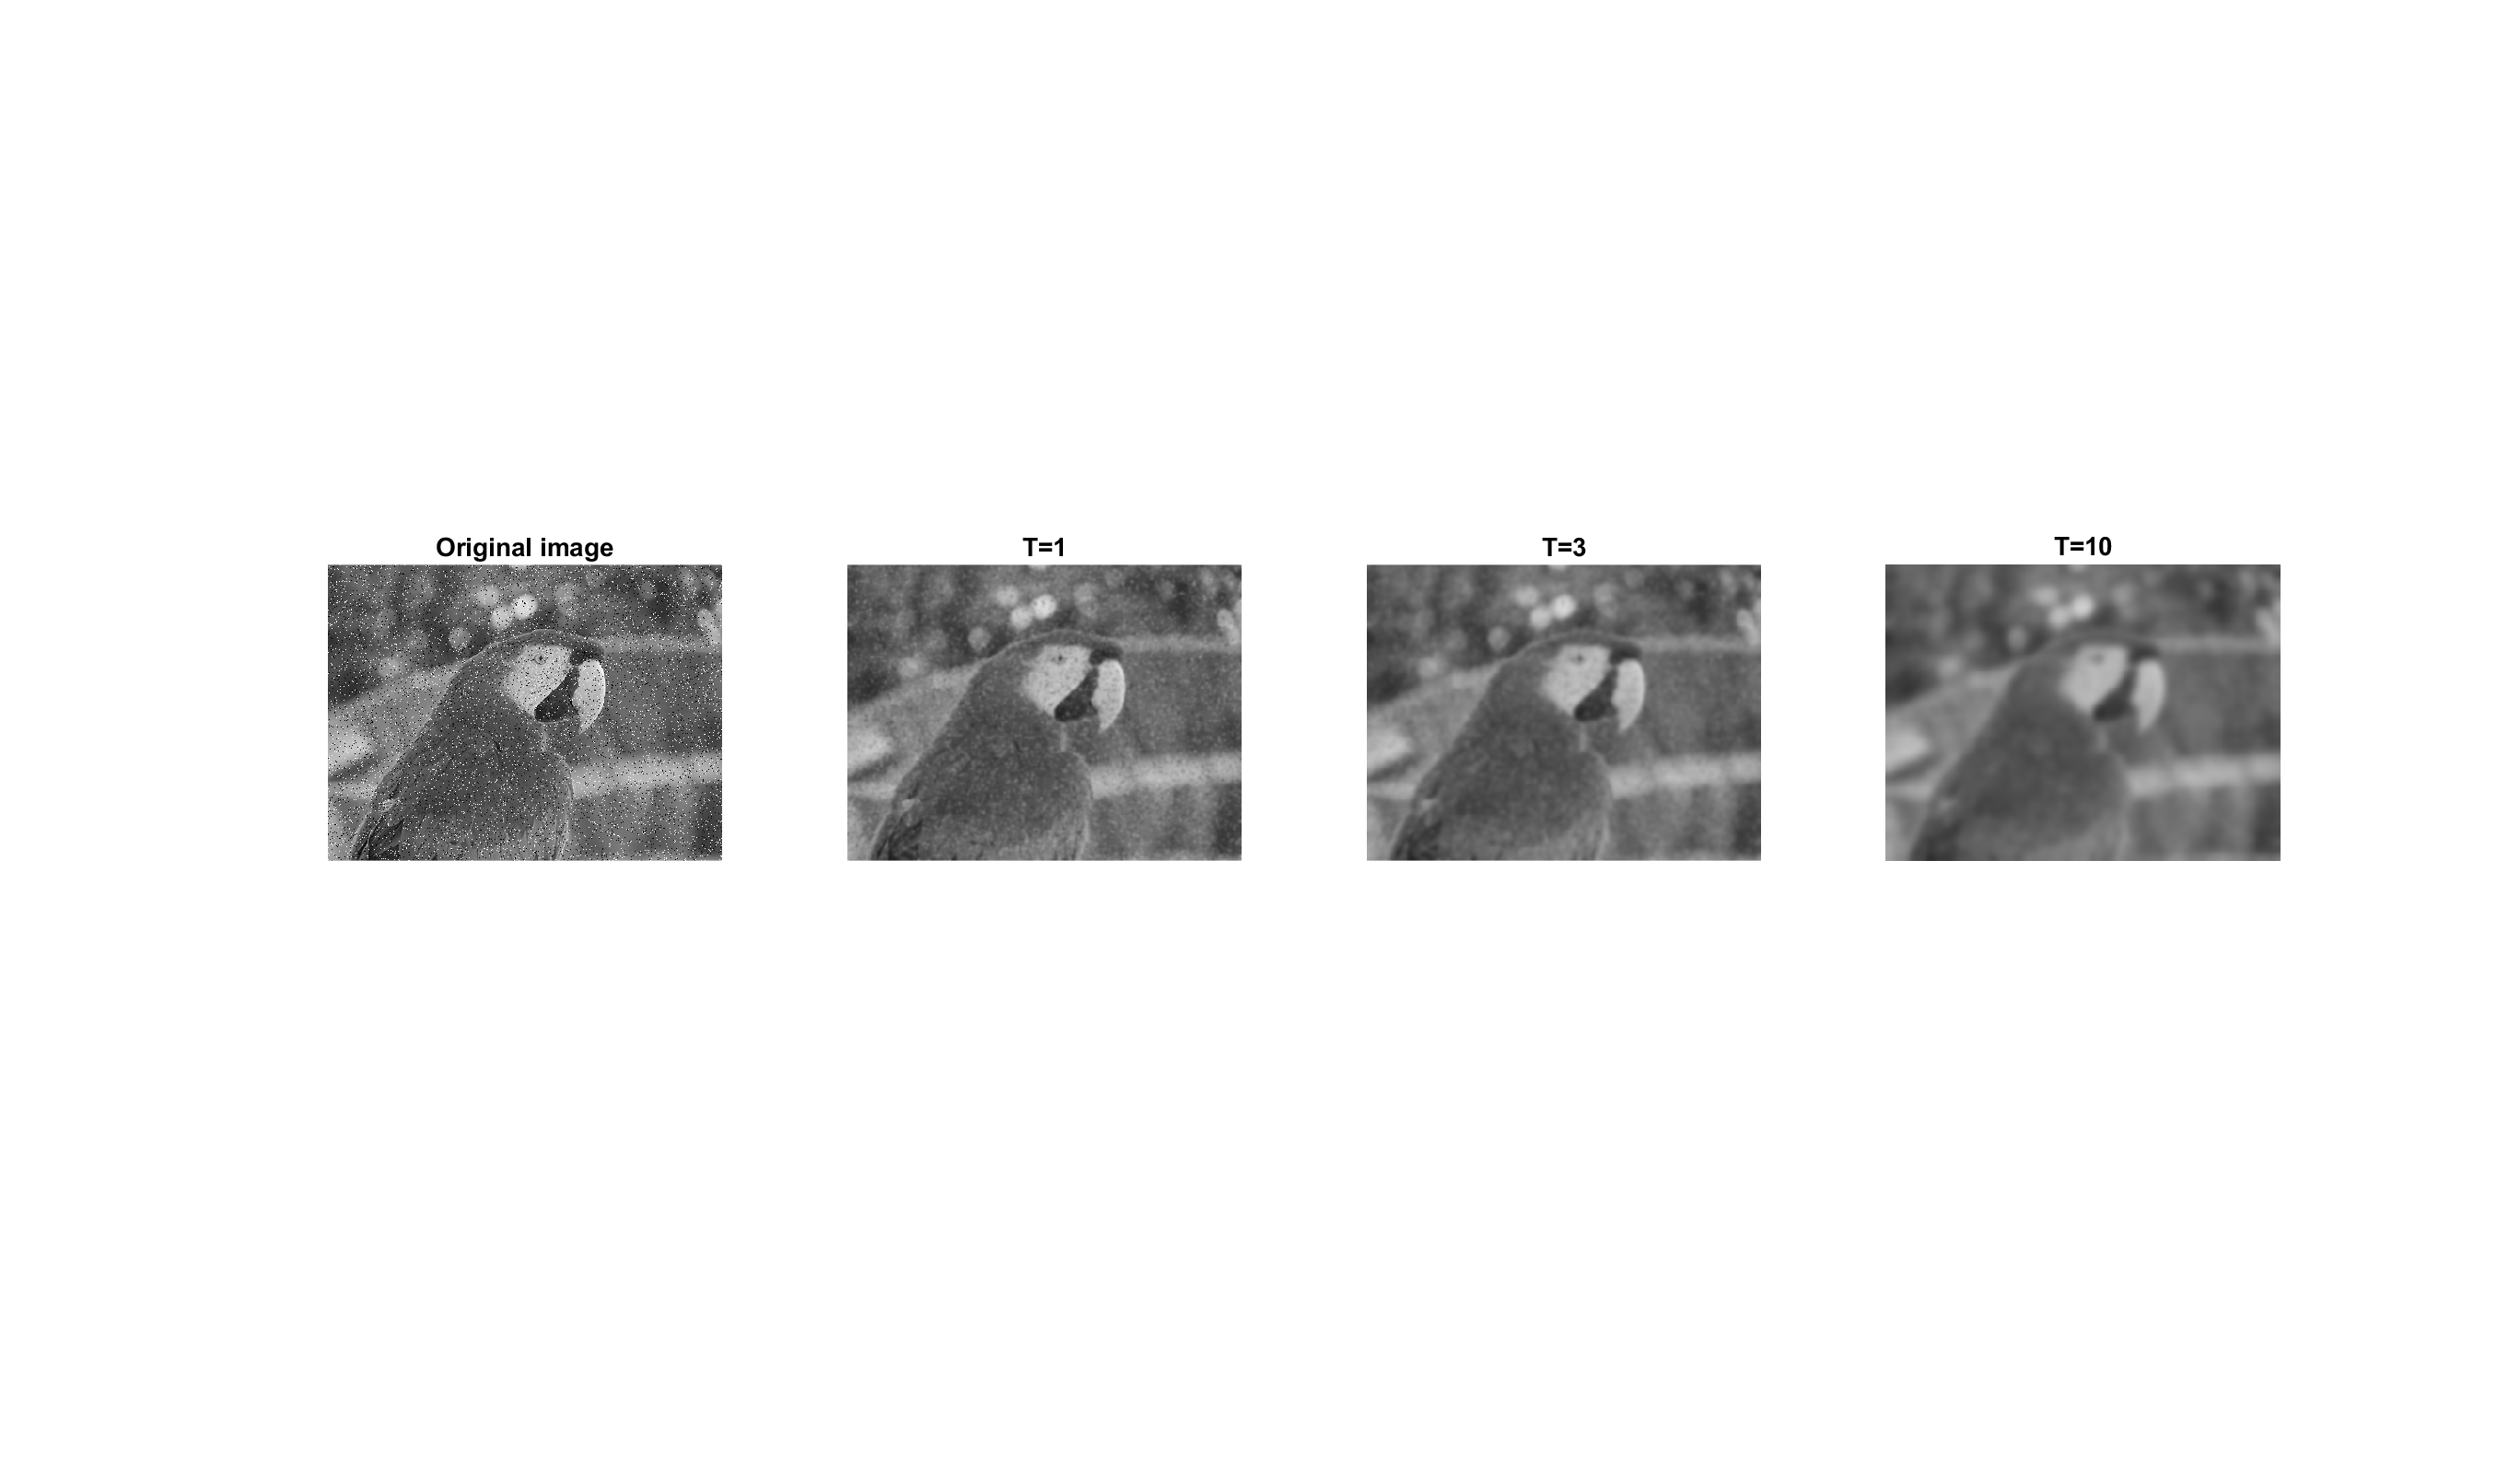
\includegraphics[scale=0.27, trim = 10.9cm 16.9cm 10.9cm 14.9cm, clip]{Pictures/Risultati/eq del calore_striscia.png}
%\includegraphics[scale=0.27, trim = 1.9cm 0.0cm 1.9cm 0.6cm, clip]{Pictures/Risultati/eq del calore 1.png}
%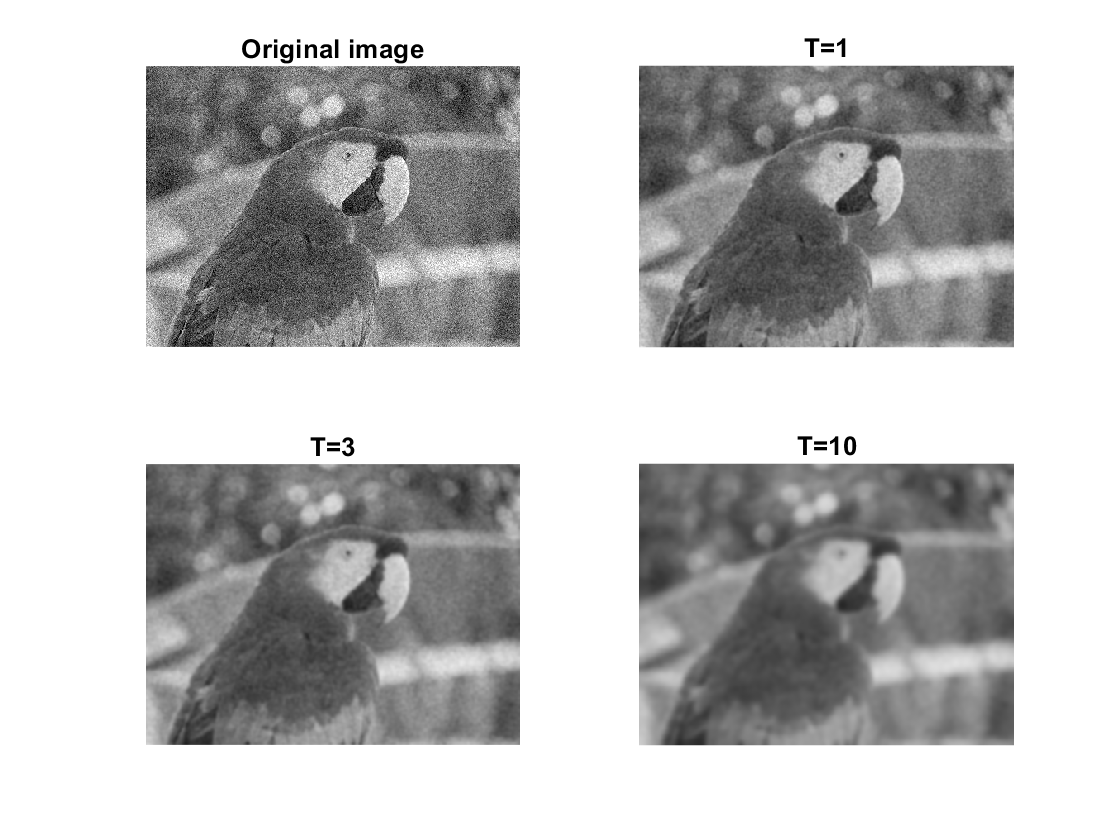
\includegraphics[scale=0.27, trim = 1.9cm 1.3cm 1.9cm 10.3cm, clip]{Pictures/Risultati/eq del calore.png}
\caption{Effetti dell'equazione del calore nel tempo.}\label{fig:figura}
\end{figure}


Questo metodo però ha un importante difetto, il rumore viene effettivamente eliminato o almeno ridotto ma si perdono importanti dettagli. Esistono procedimenti come il metodo Perona-Malik che sono decisamente più efficaci.\\


\subsection{Studio della stabilità del metodo}
Procediamo adesso ad uno studio della stabilità di tale metodo tramite il \textbf{metodo di Von Neumann}.\cite{stab}\\
Il metodo di Von Neuman si basa sulla decomposizione degli errori in serie di Fourier\\
Senza ledere di generalità, consideriamo il caso dell'equazione del calore uno-dimensionale, come visto essa può essere discretizzata come:
$$
u_{j}^{n+1}=u_{j}^{n}+r(u_{j+1}^{n}-2u_{j}^{n}+u_{j-1}^{n})
$$
dove $r=\sigma \frac{\Delta t}{(\Delta x)^2}$\\

Definiamo l'errore $\epsilon=N-u$ dove u è la soluzione calcolata dall'algoritmo in precisione infinita e N è la soluzione calcolata in precisione finita di calcolo, allora
\hspace{0.25em}
$u_{j}^{n+1}=u_{j}^{n}+r(u_{j+1}^{n}-2u_{j}^{n}+u_{j-1}^{n})$
e
$N_{j}^{n+1}=N_{j}^{n}+r(N_{j+1}^{n}-2N_{j}^{n}+N_{j-1}^{n})$
da cui 
$$
\epsilon_{j}^{n+1}=N_{j}^{n+1}-u_{j}^{n+1}=N_{j}-u_{j}^{n}+r(N_{j+1}-u_{j+1}^{n}-2N_{j}+2u_{j}^{n}+N_{j-1}-u_{j-1}^{n})=\epsilon _{j}^{n}+r(\epsilon _{j+1}^{n}-2\epsilon _{j}^{n}+\epsilon _{j-1}^{n})
$$
questo dimostra che la soluzione e l'errore hanno lo stesso andamento.\\
%Per le equazioni differenziali lineari con condizioni al contorno periodiche, la variazione spaziale dell'errore può essere espansa in una serie finita di Fourier rispetto a x nell'intervallo L, cioè
%$$
%\epsilon (x,t)=\sum _{m=-M}^{M}E_{m}(t)e^{{i}k_{m}x}
%$$
%dove $k_{m}={\frac {\pi m}{L}}$ è il numero d'onda e $M=\frac{L}{\Delta x}$

La variazione spaziale dell'errore può essere espansa con un integrale di Fourier rispetto ad x, cioè:
$$
\epsilon (x,t)=\int _{k=-{\frac {\pi }{\Delta x}}}^{k={\frac {\pi }{\Delta x}}}E_{k}(t)e^{{i}kx}dk
$$
Essendo l'equazione lineare, il termine generico va come l'integrale stesso, ossia: 
$\epsilon _{j}^{n}=E_{m}(t)e^{ik_{m}x}$ da cui:\\
\vspace{0.5em}
$\epsilon _{j}^{n+1}=E_{m}(t+\Delta t)e^{ik_{m}x}$\\ 
$\epsilon _{j+1}^{n}=E_{m}(t)e^{ik_{m}(x+\Delta x)}$\\ 
$\epsilon _{j-1}^{n}=E_{m}(t)e^{ik_{m}(x-\Delta x)}$\\
Sostituindo questi valori in $\epsilon_{j}^{n+1}=\epsilon _{j}^{n}+r(\epsilon _{j+1}^{n}-2\epsilon _{j}^{n}+\epsilon _{j-1}^{n})$ si ottiene:

$$
E_{m}(t+\Delta t)e^{ik_{m}x}=E_{m}(t)e^{ik_{m}x}+r(E_{m}(t)e^{ik_{m}(x+\Delta x)}-2E_{m}(t)e^{ik_{m}x}+E_{m}(t)e^{ik_{m}(x-\Delta x)})
$$
Affinché il metodo sia stabile occorre che l'errore non aumenti mai, ossia che\\
\vspace{0.25em}
$|E_{m}(t+\Delta t)|\leq |E_{m}(t)| \Rightarrow |\frac{E_{m}(t+\Delta t)}{E_{m}(t)}|\leq 1$. Esplicitiamo quindi per $\frac{E_{m}(t+\Delta t)}{E_{m}(t)}$ ed otteniamo:

$$
\frac {E_{m}(t+\Delta t)}{E_{m}(t)}=1+r(e^{ik_{m}\Delta x}+e^{-ik_{m}\Delta x}-2).
$$
detto $\theta =k_{m}\Delta x$, ricordo $k\in [\frac{\pi}{\Delta x},-\frac{\pi}{\Delta x}]$ per cui $\theta \in [-\pi ,\pi ]$
per cui l'equazione diventa
$$
\frac {E_{m}(t+\Delta t)}{E_{m}(t)}=1+r(e^{i\theta x}+e^{-i\theta}-2).
$$

Prendiamo ora in considerazione l'identità 
$$
\sin \left({\frac {\theta }{2}}\right)={\frac {e^{i\theta /2}-e^{-i\theta /2}}{2i}} \Rightarrow
\sin ^{2}\left({\frac {\theta }{2}}\right)=-{\frac {e^{i\theta }+e^{-i\theta }-2}{4}}
$$
alla luce di questa osservazione, l'equazione diventa:
$$
\frac {E_{m}(t+\Delta t)}{E_{m}(t)}=1-4r\sin^2(\frac{\theta}{2}).
$$

Come detto, il metodo è stabile $\Leftrightarrow|\frac{E_{m}(t+\Delta t)}{E_{m}(t)}|\leq 1$ ma visto che $\frac {E_{m}(t+\Delta t)}{E_{m}(t)}=1-4r\sin^2(\frac{\theta}{2})\Rightarrow$ il metodo risulta stabile $\Leftrightarrow|1-4r\sin^2(\frac{\theta}{2})|\leq1$. Esplicitando:
$$
-1\leq 1-4r\sin^2(\frac{\theta}{2})\leq 1 \Rightarrow-2\leq -4r\sin^2(\frac{\theta}{2})\leq 0 \Rightarrow 0\leq 4r\sin^2(\frac{\theta}{2})\leq 2
$$
ma $\sin^2(\frac{\theta}{2})\ge0$ $\forall\theta\Rightarrow$il metodo risulta stabile $\Leftrightarrow r\sin^2(\frac{\theta}{2})\leq\frac{1}{2}$ siccome $\sin^2(\frac{\theta}{2})\leq1$ $\forall\theta\Rightarrow$ la condizione è sicuramente soddisfatta se $r\leq\frac{1}{2}$.
Avendo definito $r=\sigma \frac{\Delta t}{(\Delta x)^2} \Rightarrow$ condizione sufficiente affinché il metodo sia stabile è $\sigma \frac{\Delta t}{(\Delta x)^2}\leq\frac{1}{2}$\\
\vspace{1em}
Nel caso 2-dimensionale la soluzione discreta della PDE è:
$$
u_{j,k}^{n+1}=u_{j,k}^{n}+r_{x}(u_{j+1,k}^{n}-2u_{j,k}^{n}+u_{j-1,k}^{n})+r_{y}(u_{j,k+1}^{n}-2u_{j,k}^{n}+u_{j,k-1}^{n})
$$
dove $r_{x}=\sigma \frac{\Delta t}{(\Delta x)^2}$ e $r_{y}=\sigma \frac{\Delta t}{(\Delta y)^2}$\\ per cui la condizione diventa $r_{x}+r_{y}=\sigma \frac{\Delta t}{(\Delta x)^2}+\sigma \frac{\Delta t}{(\Delta y)^2}\leq\frac{1}{2}$.\\
Nel caso in esame $\Delta x=\Delta y=1 \Rightarrow r_{x}+r_{y}=\sigma \Delta t+\sigma \Delta t\leq\frac{1}{2} \Rightarrow \sigma\Delta t\leq \frac{1}{4}$

